\section{ANEXOS}

\subsection{ANEXO A: DIAGRAMA DE BLOQUES DEL SEP}

\begin{center}
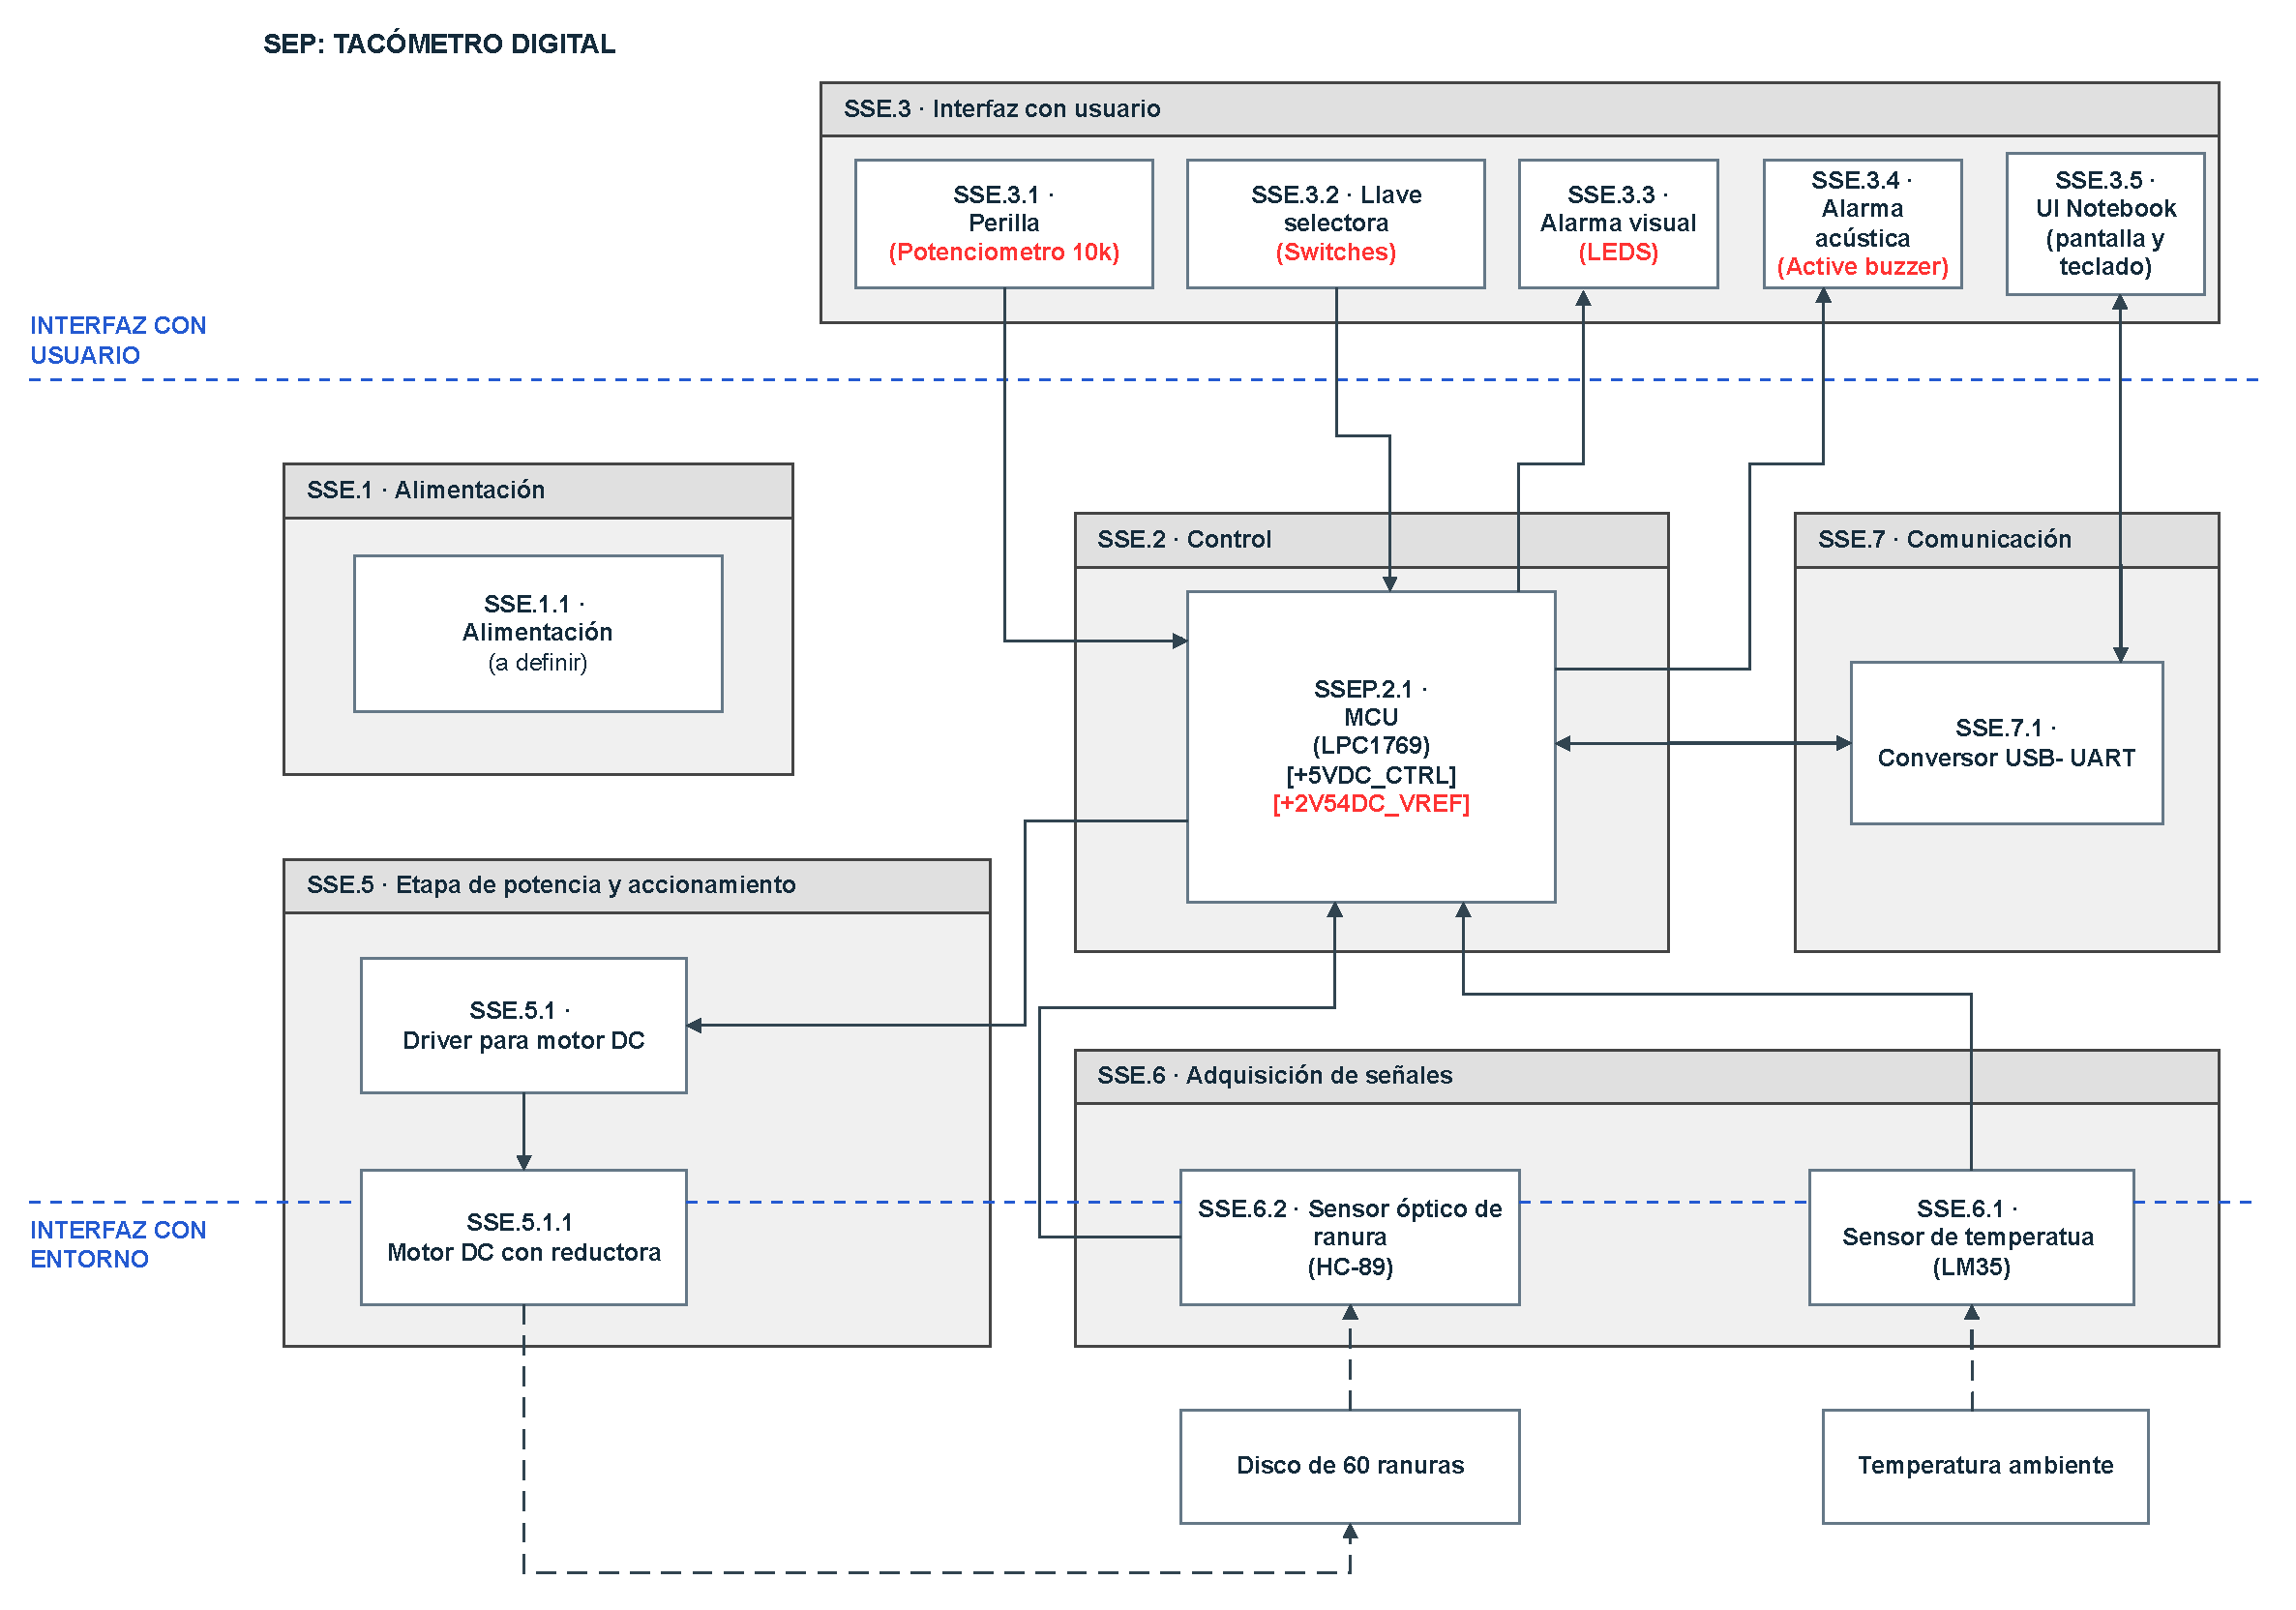
\includegraphics[width=\textwidth,height=0.75\textheight,keepaspectratio]{diagramas/hardware.pdf}
\end{center}

\pendiente{volver a exportar hardware.pdf desde hardware.drawio (ya actualizado con
XD-51 y VREFP 3,3\,V; falta completar la alimentación)}.

\clearpage
\subsection{ANEXO B: FIRMWARE DEL SEP}

\begin{center}
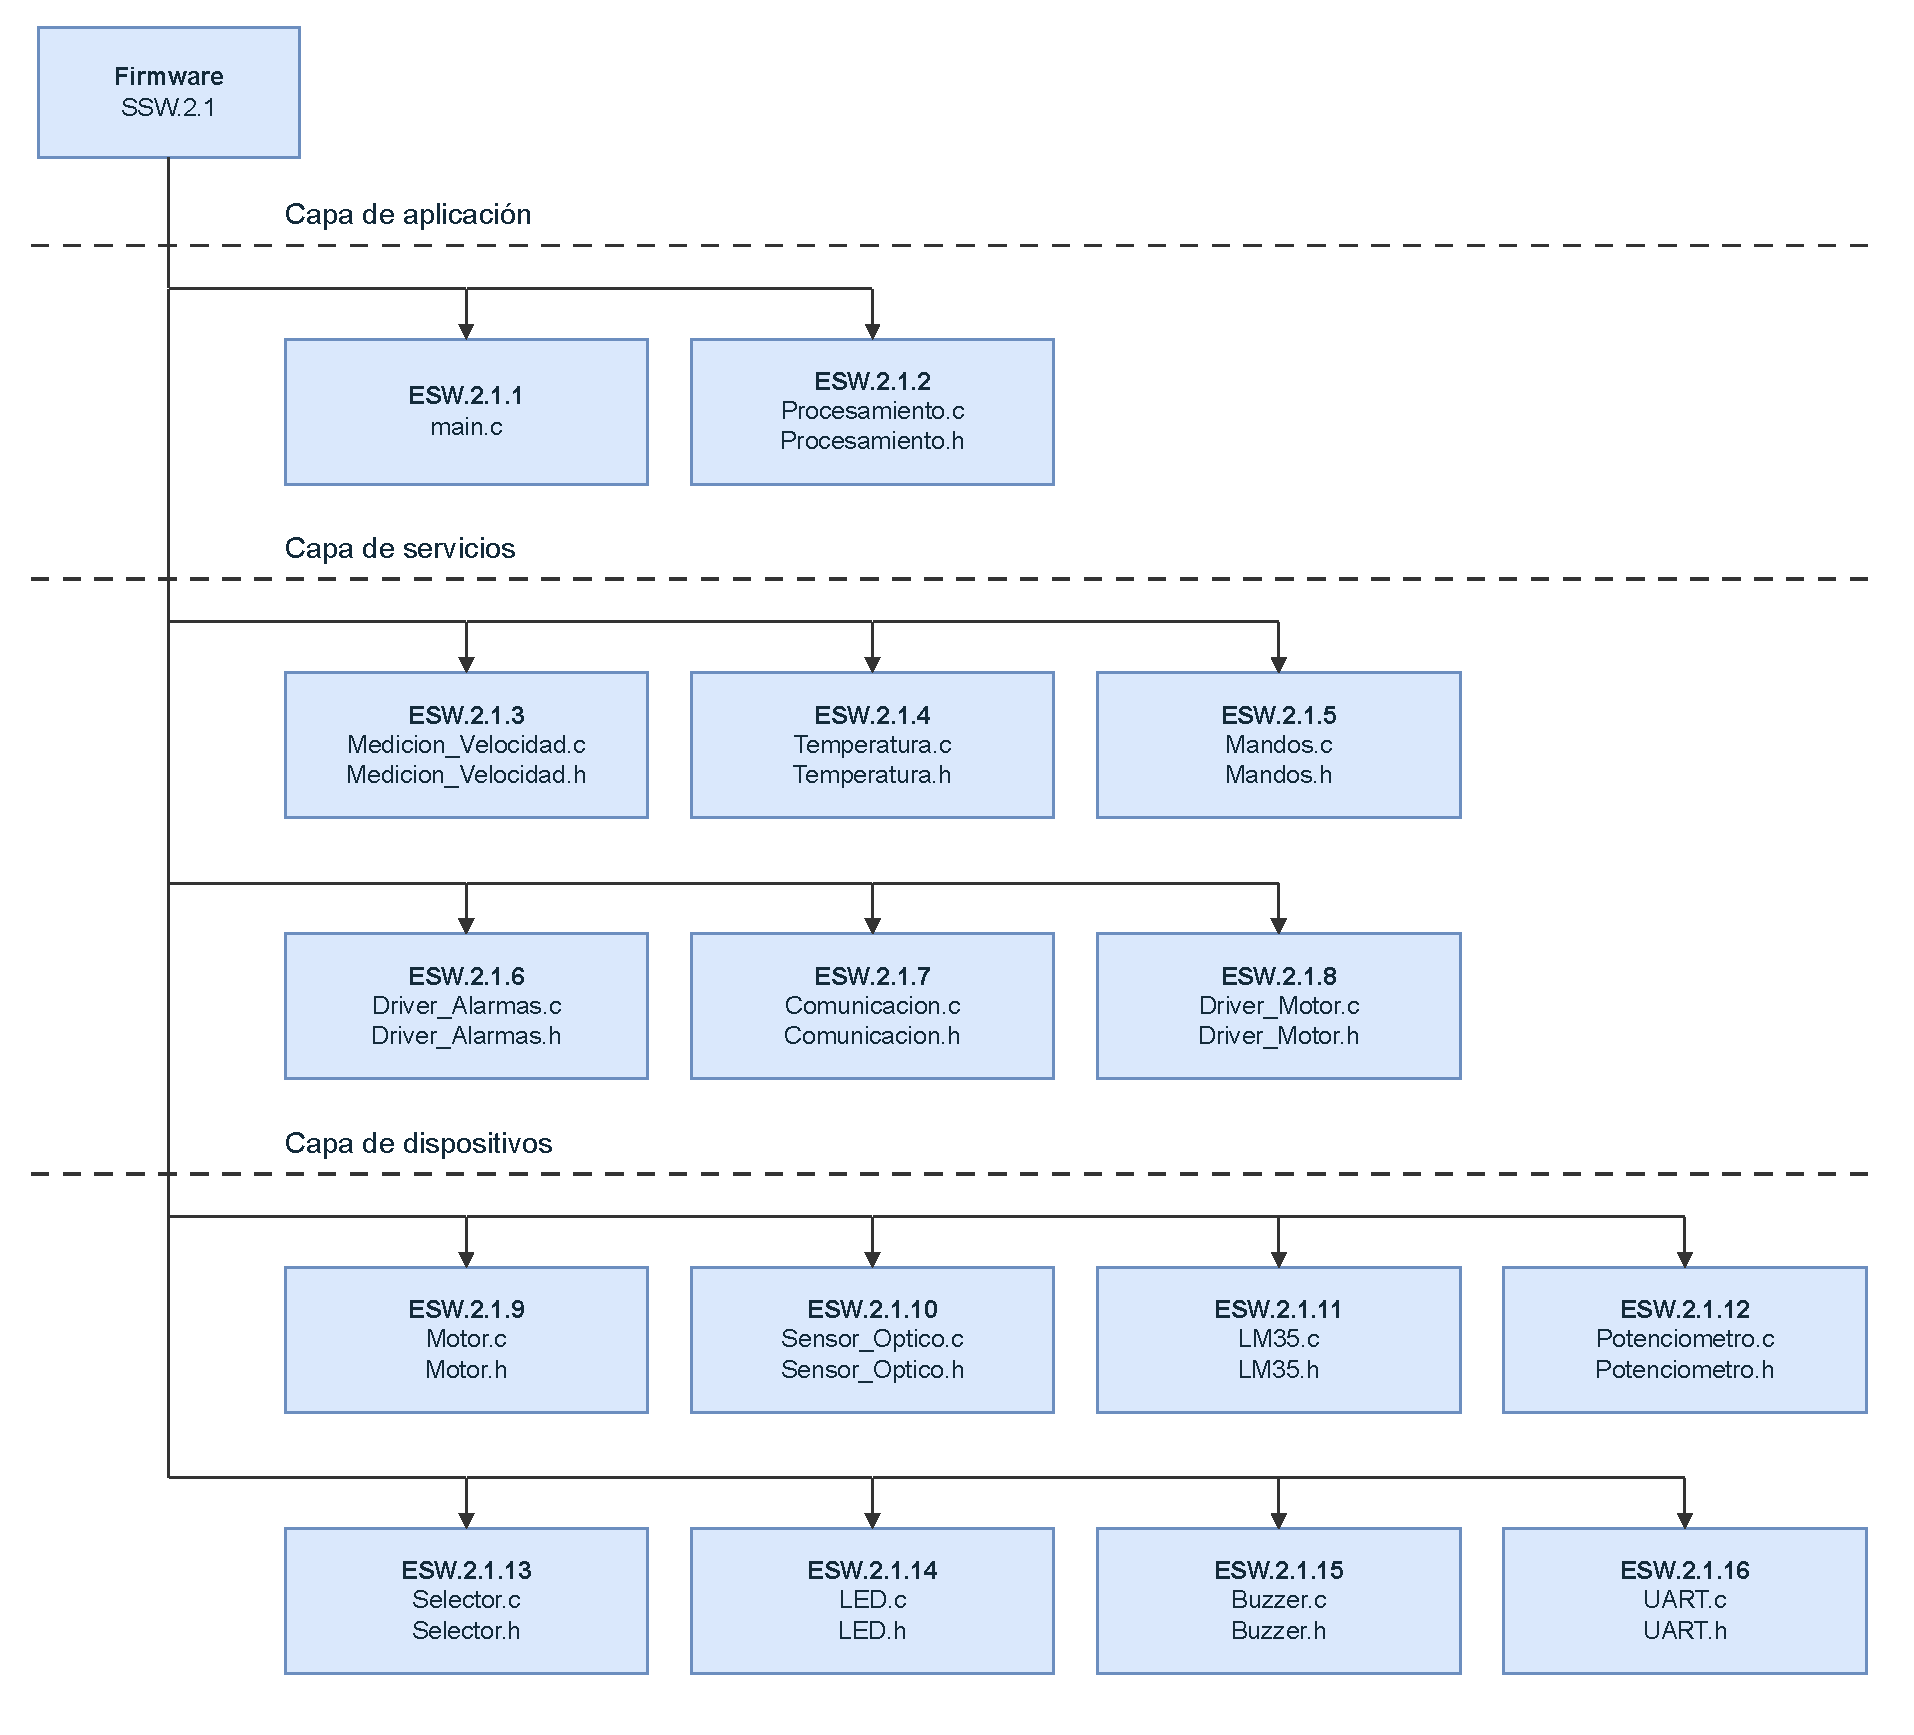
\includegraphics[width=\textwidth,height=0.75\textheight,keepaspectratio]{diagramas/firmware.pdf}
\end{center}

Los módulos de soporte de plataforma (Sistema, Reloj y Adquisicion\_ADC\_DMA), sin ESW
propio, se indican con borde punteado.
\pendiente{volver a exportar firmware.pdf desde firmware.drawio (ya actualizado con
ESW.2.1.17 y el soporte de plataforma)}.

\subsubsection{SECUENCIA DEL PERÍODO DE CONTROL}

La siguiente secuencia muestra cómo cooperan las capas en cada período de 500\,ms, en
modo automático con consigna activa:

\begin{enumerate}
  \item \texttt{TIMER0\_IRQHandler} (dispositivos) cierra la ventana: lee
  \texttt{SensorOptico\_Read} y publica los pulsos.
  \item \texttt{Aplicacion\_Iterar} llama a \texttt{Medicion\_Velocidad\_Actualizar}
  (servicios), que obtiene los pulsos con \texttt{Timer\_ConsumirVentana} y devuelve la
  velocidad en milésimas de RPM.
  \item \texttt{Aplicacion\_Periodo} llama a \texttt{Temperatura\_Leer} $\rightarrow$
  \texttt{LM35\_Read}; la decisión de \texttt{Procesamiento\_EvaluarAlarma} se aplica con
  \texttt{Driver\_Alarmas\_Aplicar} $\rightarrow$ \texttt{LED\_Write} y
  \texttt{Buzzer\_Write}.
  \item Lee las consignas con \texttt{Comunicacion\_RecibirConsigna} $\rightarrow$
  \texttt{UART\_Read} y la llave con \texttt{Mandos\_LeerModo} $\rightarrow$
  \texttt{Selector\_Read}; \texttt{Procesamiento\_ActualizarModo} devuelve el estado.
  \item \texttt{Procesamiento\_Regular} calcula el mando, que se aplica con
  \texttt{Driver\_Motor\_Aplicar} $\rightarrow$ \texttt{Motor\_Write}.
  \item \texttt{Comunicacion\_EnviarTelemetria} arma la trama y la encola con
  \texttt{UART\_Write}; \texttt{UART3\_IRQHandler} la transmite en segundo plano.
\end{enumerate}

\subsection{ANEXO C: CÓDIGO FUENTE}

El código fuente completo, documentado con Doxygen, se entrega en la carpeta
\texttt{Firmware/} y está disponible en el repositorio del proyecto.
